\subsubsection{Overview}
\label{Spike Statistics}
\index{Spike Statistics}\index{utilities, Spike Statistics}
\begin{figure}[h]
\begin{center}
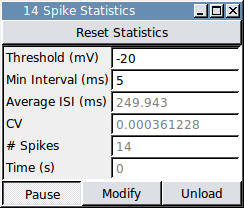
\includegraphics[width=2in]{spikestatistics.png} 
\caption[Spike Statistics]{The spike statistics module monitors the spike 
'state' based on user-defined parameters and calculates the average interval between spikes.} 
\end{center}
\label{spikestatistics}
\end{figure}

This module contains a spike detector based on a positive threshold crossing (see SpikeDetect module). It computes the average ISI and the current coefficient of variation. These values are continuously updated with each spike until the statistics are reset with the button.

\subsubsection{Input Channels}
\begin{description}
\item[input(0)- "Vm" (mV)] the membrane potential
\end{description}

\subsubsection{Output Channels}
\begin{description}
\item[output(0) - "ISI"] Output current (A)
\end{description}

\subsubsection{Parameters}
\begin{description}
\item[Threshold (mV)] the threshold at which a spike is detected
\item[Min. Interval (ms)] minimum interval (refractory period) that must pass before another spike can be detected
\end{description}